\documentclass[tikz,border=5pt]{standalone}
\usepackage{pgfplots}
\usepackage[dvipsnames]{xcolor}
\pgfplotsset{compat=1.17}

\definecolor{gold}{HTML}{CFB87C}
\definecolor{blue}{HTML}{156082}
\definecolor{green}{HTML}{196B24}
\definecolor{orange}{HTML}{E97132}
\definecolor{dkgray}{HTML}{333333}
\definecolor{ltgray}{HTML}{D9D9D9}

\begin{document}
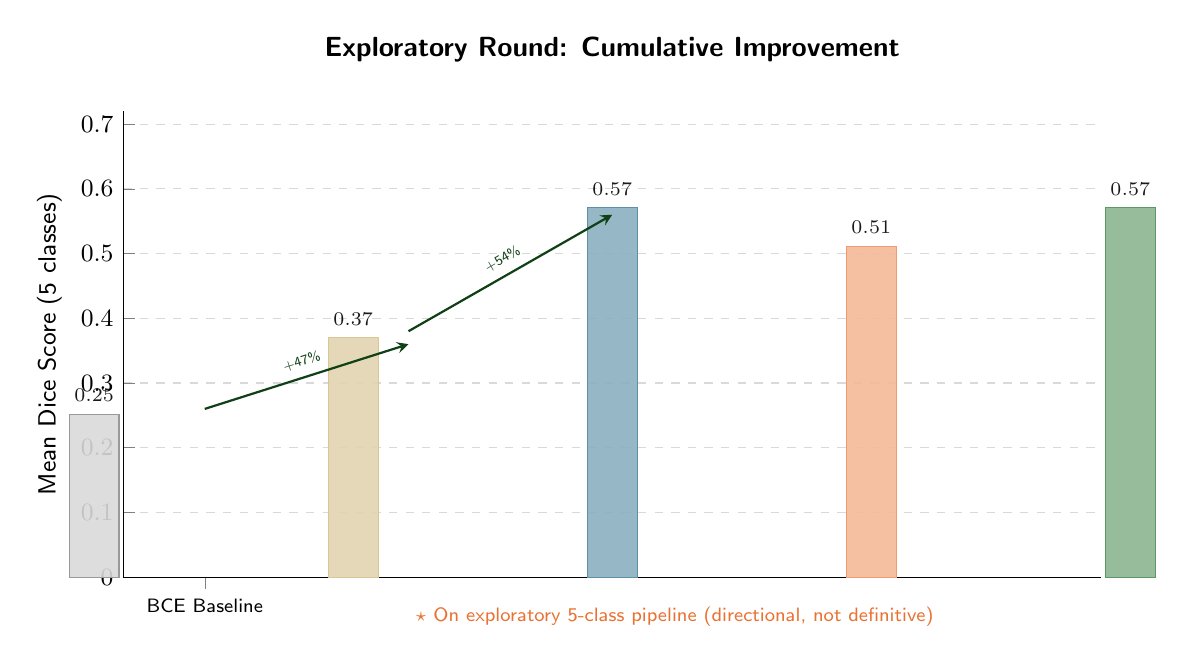
\begin{tikzpicture}
\begin{axis}[
    ybar,
    width=14cm,
    height=7.5cm,
    bar width=18pt,
    ylabel={Mean Dice Score (5 classes)},
    ylabel style={font=\sffamily\small},
    xtick=data,
    symbolic x coords={BCE Baseline, {+Tversky ($\alpha$=0.6)}, {+Balanced Softmax}, {+Foreground Fix}, {+MaskSup 0.3}},
    xticklabel style={font=\sffamily\scriptsize, rotate=0, anchor=north, align=center, text width=2.5cm},
    yticklabel style={font=\sffamily\small},
    ymin=0, ymax=0.72,
    ytick={0, 0.1, 0.2, 0.3, 0.4, 0.5, 0.6, 0.7},
    nodes near coords,
    nodes near coords style={font=\sffamily\scriptsize\bfseries, above, yshift=1pt},
    nodes near coords align={vertical},
    every axis plot/.append style={fill opacity=0.9},
    legend style={at={(0.98,0.95)}, anchor=north east, font=\sffamily\footnotesize, draw=none, fill=white, fill opacity=0.8},
    axis lines*=left,
    ymajorgrids=true,
    grid style={dashed, gray!30},
    clip=false,
    title={\textbf{Exploratory Round: Cumulative Improvement}},
    title style={font=\sffamily\normalsize, at={(0.5,1.05)}},
]

% Bars with increasing color intensity
\addplot[fill=ltgray, draw=dkgray!50] coordinates {
    (BCE Baseline, 0.252)
};
\addplot[fill=gold!60, draw=gold!80] coordinates {
    ({+Tversky ($\alpha$=0.6)}, 0.370)
};
\addplot[fill=blue!50, draw=blue!70] coordinates {
    ({+Balanced Softmax}, 0.571)
};
\addplot[fill=orange!50, draw=orange!70] coordinates {
    ({+Foreground Fix}, 0.511)
};
\addplot[fill=green!50, draw=green!70] coordinates {
    ({+MaskSup 0.3}, 0.571)
};

% Improvement annotations
\draw[-{stealth}, thick, green!60!black] (axis cs:BCE Baseline, 0.26) -- 
    node[above, font=\sffamily\tiny, text=green!60!black, sloped] {+47\%}
    (axis cs:{+Tversky ($\alpha$=0.6)}, 0.36);

\draw[-{stealth}, thick, green!60!black] (axis cs:{+Tversky ($\alpha$=0.6)}, 0.38) -- 
    node[above, font=\sffamily\tiny, text=green!60!black, sloped] {+54\%}
    (axis cs:{+Balanced Softmax}, 0.56);

\end{axis}

% Caveat note
\node[font=\sffamily\scriptsize, text=orange, align=left] at (7, -0.5) {%
    $\star$ On exploratory 5-class pipeline (directional, not definitive)%
};

\end{tikzpicture}
\end{document}
